\documentclass[9pt,aspectratio=169,xcolor=table]{beamer}

%~~~~~~~~~~~~~~~~~~~~~~~~~~~~~~~~~~~~~~~~~~~~~~~~~~~~~~~~~~~~~~~~~~~~~~~~~~~~~~
% Use roboto Font (recommended)
\usepackage[sfdefault]{roboto}
\usepackage[utf8]{inputenc}
\usepackage[T1]{fontenc}
%~~~~~~~~~~~~~~~~~~~~~~~~~~~~~~~~~~~~~~~~~~~~~~~~~~~~~~~~~~~~~~~~~~~~~~~~~~~~~~

%~~~~~~~~~~~~~~~~~~~~~~~~~~~~~~~~~~~~~~~~~~~~~~~~~~~~~~~~~~~~~~~~~~~~~~~~~~~~~~
% Define where theme files are located. ('/styles')
\usepackage{styles/fluxmacros}
\usefolder{styles}
% Use Flux theme v0.1 beta
% Available style: asphalt, blue, red, green, gray
% "red" is the closest built-in style to maroon; its exact colours are
% overridden with a true maroon palette just below, after the theme loads.
\usetheme[style=red]{flux}
%~~~~~~~~~~~~~~~~~~~~~~~~~~~~~~~~~~~~~~~~~~~~~~~~~~~~~~~~~~~~~~~~~~~~~~~~~~~~~~

%~~~~~~~~~~~~~~~~~~~~~~~~~~~~~~~~~~~~~~~~~~~~~~~~~~~~~~~~~~~~~~~~~~~~~~~~~~~~~~
% SKEE1033 maroon palette override.
% The flux theme's colortheme defines primaryLight/primary/secondary/tertiary
% as plain \definecolor calls (not \providecolor), so simply redefining them
% here, AFTER \usetheme, wins -- xcolor allows redefinition and every
% \setbeamercolor in beamercolorthemeflux.sty was already evaluated against
% these names, so the redefinition propagates everywhere automatically.
\definecolor{primaryLight}{HTML}{9B2242} % lighter maroon -- headers, accents
\definecolor{primary}{HTML}{7B1E3A}      % core maroon -- titles, block headers
\definecolor{secondary}{HTML}{3A5A6B}    % muted teal -- complementary accent
\definecolor{tertiary}{HTML}{8C6A3F}     % warm bronze -- example/third accent
%~~~~~~~~~~~~~~~~~~~~~~~~~~~~~~~~~~~~~~~~~~~~~~~~~~~~~~~~~~~~~~~~~~~~~~~~~~~~~~

%~~~~~~~~~~~~~~~~~~~~~~~~~~~~~~~~~~~~~~~~~~~~~~~~~~~~~~~~~~~~~~~~~~~~~~~~~~~~~~
% Extra packages
\usepackage{booktabs}
\usepackage{colortbl}
\usepackage{ragged2e}
\usepackage{amssymb}
\usepackage{multirow}
\usepackage{tikz}
\usetikzlibrary{arrows.meta, positioning, fit, backgrounds, calc, shapes.geometric}
\setbeamertemplate{itemize items}[square]
\usepackage[scaled=.92]{beramono}
\usepackage{listings}
\usepackage{array}
% Table striping: odd rows white, even rows very light gray.
\definecolor{stripe}{gray}{0.94}
\newcommand{\striped}{\rowcolors{1}{white}{stripe}}
%~~~~~~~~~~~~~~~~~~~~~~~~~~~~~~~~~~~~~~~~~~~~~~~~~~~~~~~~~~~~~~~~~~~~~~~~~~~~~~

%~~~~~~~~~~~~~~~~~~~~~~~~~~~~~~~~~~~~~~~~~~~~~~~~~~~~~~~~~~~~~~~~~~~~~~~~~~~~~~
% Code listing style (lightweight analogue of the book's skpython style).
% This course is Python-only, so Python is set as the lstlisting default via
% \lstset below -- every \begin{lstlisting} needs no language=... of its own.
\definecolor{codebg}{HTML}{FBF2F4}
\definecolor{codegreen}{rgb}{0,0.45,0}
\definecolor{codestring}{rgb}{0.58,0.1,0.2}
\lstdefinestyle{skpython}{
    basicstyle=\ttfamily\footnotesize,
    keywordstyle=\color{primary}\bfseries,
    commentstyle=\itshape\color{codegreen},
    stringstyle=\ttfamily\color{codestring},
    backgroundcolor=\color{codebg},
    breaklines=true,
    keepspaces=true,
    showspaces=false,
    showstringspaces=false,
    frame=single,
    rulecolor=\color{primary!40},
    numbers=none,
}
\lstset{language=Python, style=skpython}
%~~~~~~~~~~~~~~~~~~~~~~~~~~~~~~~~~~~~~~~~~~~~~~~~~~~~~~~~~~~~~~~~~~~~~~~~~~~~~~

%~~~~~~~~~~~~~~~~~~~~~~~~~~~~~~~~~~~~~~~~~~~~~~~~~~~~~~~~~~~~~~~~~~~~~~~~~~~~~~
% TikZ block styles for the computation-cycle diagram and OOP class/object
% boxes. oop* styles mirror the book's own naming (chapter15.tex) so figures
% can be ported between book and slides with only colour changes.
\definecolor{cycfill}{HTML}{F3DCE4}
\definecolor{cycline}{HTML}{7B1E3A}
\definecolor{cycdofill}{HTML}{E8EEF0}
\definecolor{cycdoline}{HTML}{3A5A6B}
\tikzset{
  cycstep/.style = {font=\sffamily\small, align=center, rounded corners=2pt,
                     draw=cycline, fill=cycfill, line width=0.7pt,
                     minimum height=7mm, minimum width=20mm, inner sep=3pt},
  cycdo/.style   = {cycstep, fill=cycdofill, draw=cycdoline},
  flow/.style    = {-{Stealth[length=2mm]}, thick, draw=cycline},
  oopttl/.style  = {font=\sffamily\bfseries\small, align=center,
                     rounded corners=2pt, draw=primary, fill=primary!18,
                     line width=0.7pt, minimum height=6mm, inner sep=3pt},
  oopdata/.style = {font=\sffamily\scriptsize, align=left,
                     draw=tertiary, fill=tertiary!14,
                     line width=0.7pt, minimum height=5mm, inner sep=3pt},
  oopmeth/.style = {font=\sffamily\scriptsize, align=left,
                     draw=primary, fill=primary!8,
                     line width=0.7pt, minimum height=5mm, inner sep=3pt},
  ooparr/.style  = {draw=black!65, line width=0.7pt,
                     -{Latex[length=2.0mm]}},
  oopinh/.style  = {draw=primary, line width=0.8pt,
                     -{Triangle[open, length=2.6mm, width=2.6mm]}},
  ooplbl/.style  = {font=\sffamily\scriptsize\itshape, text=black!65,
                     inner sep=2pt},
}
%~~~~~~~~~~~~~~~~~~~~~~~~~~~~~~~~~~~~~~~~~~~~~~~~~~~~~~~~~~~~~~~~~~~~~~~~~~~~~~

%%%%%%%%%%%%%%%%%%%%%%%%%%%%%%%%%%%
%% SECTION SEPARATOR (ToC recap) %%
%%%%%%%%%%%%%%%%%%%%%%%%%%%%%%%%%%%
\AtBeginSection[]
{
{
    \setbeamercolor{background canvas}{bg=primaryLight!6}
    \begin{frame}[plain]
        \frametitle{Table of Contents}
        \tableofcontents[currentsection]
    \end{frame}
}
}
%%%%%%%%%%%%%%%%%%%%%%%%%%%%%%%%%%%

%~~~~~~~~~~~~~~~~~~~~~~~~~~~~~~~~~~~~~~~~~~~~~~~~~~~~~~~~~~~~~~~~~~~~~~~~~~~~~~
% Information
\title{A First Look at Object-Oriented Python}
\subtitle{\emph{Engineering Computation with Python} --- Chapter 15}
\author{Mun\'{i}m Zabidi}
\institute{\color{primary}Faculty of Electrical Engineering, Universiti Teknologi Malaysia}
\date{\today}
\titlegraphic{assets/logoutmwhite.png}
%~~~~~~~~~~~~~~~~~~~~~~~~~~~~~~~~~~~~~~~~~~~~~~~~~~~~~~~~~~~~~~~~~~~~~~~~~~~~~~

\begin{document}

\titlepage

\begin{frame}{Table of Contents}
    \tableofcontents
\end{frame}

%===============================================================================
\section{Why Objects?}
%===============================================================================

\begin{frame}{An Enrichment Chapter}
    \leavevmode
    \small
    \begin{alertblock}{Not a taught week}
        Roughly three lecture hours. This chapter is deliberately brief ---
        Python's object system is large, and most of it is not needed for
        engineering computation.
    \end{alertblock}

    \vspace{3mm}
    By the end, you should be able to:
    \begin{itemize}\itemsep1pt
        \item Explain what a class and an object are, and how they differ.
        \item Define a class with \texttt{\_\_init\_\_} and store data in
              attributes.
        \item Write methods that operate on an object's own data via
              \texttt{self}.
        \item Use inheritance to share behaviour between related classes.
        \item Recognise that NumPy arrays and pandas DataFrames are
              themselves objects.
    \end{itemize}
\end{frame}

\begin{frame}[fragile]{The Problem: Data and Functions, Kept Apart}
    \leavevmode
    The bench recording, handled the way earlier chapters taught it:

\begin{lstlisting}
t = ...            # the time axis
v = ...            # the voltage samples
n_missing = count_missing(v)
v = repair_gaps(t, v)
tau = fit_time_constant(t, v)
\end{lstlisting}

    \vspace{1mm}
    \begin{block}{Nothing is wrong with this \ldots}
        \ldots but nothing \alert{enforces} it either. Nothing stops you
        passing the wrong time axis to \texttt{repair\_gaps()}, or losing
        track of which of three recordings \texttt{v} currently is. The
        rules live only in the programmer's own carefulness.
    \end{block}
\end{frame}

\begin{frame}[fragile]{The Idea: Bundle Data and Behaviour}
    \leavevmode
    An \alert{object} bundles the time axis, the samples, and the
    operations that make sense on them into one thing:

\begin{lstlisting}
rc = Signal(t, v, name="bench_rc voltage")
rc.repair()
tau = rc.time_constant()
\end{lstlisting}

    \vspace{2mm}
    \begin{block}{What changed}
        \texttt{rc.repair()} \alert{cannot} be given the wrong time axis
        --- it uses the one stored inside \texttt{rc}. The recording now
        carries its own operations with it.
    \end{block}
\end{frame}

\begin{frame}{Procedural vs.\ Object-Oriented}
    \leavevmode
    \begin{columns}[t]
        \begin{column}{.5\textwidth}
            \begin{block}{Procedural}
                \small Data and functions are separate. \alert{Any}
                function can be applied to \alert{any} data --- including
                the wrong pairing.
            \end{block}
            \vspace{2mm}
            \begin{center}
            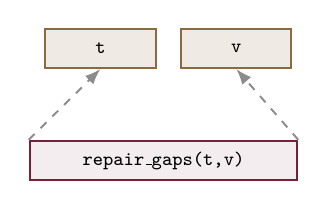
\begin{tikzpicture}[node distance=4mm]
                \node[oopdata, minimum width=14mm] (t) {\texttt{t}};
                \node[oopdata, right=3mm of t, minimum width=14mm] (v) {\texttt{v}};
                \node[oopmeth, below=9mm of t, minimum width=34mm, xshift=8mm]
                     (f1) {\texttt{repair\_gaps(t,v)}};
                \draw[ooparr, dashed, draw=black!45] (f1.north west) -- (t.south);
                \draw[ooparr, dashed, draw=black!45] (f1.north east) -- (v.south);
            \end{tikzpicture}
            \end{center}
        \end{column}
        \begin{column}{.5\textwidth}
            \begin{block}{Object-oriented}
                \small The object's boundary decides what may be applied
                to what. Methods can only reach their \alert{own} data.
            \end{block}
            \vspace{2mm}
            \begin{center}
            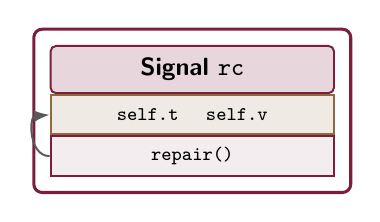
\begin{tikzpicture}
                \node[oopttl, minimum width=36mm] (ttl) {Signal \texttt{rc}};
                \node[oopdata, below=0mm of ttl, minimum width=36mm, anchor=north]
                     (d) {\texttt{self.t} \quad \texttt{self.v}};
                \node[oopmeth, below=0mm of d, minimum width=36mm, anchor=north]
                     (m) {\texttt{repair()}};
                \draw[ooparr] (m.west) to[out=180,in=185,looseness=1.3] (d.west);
                \begin{scope}[on background layer]
                    \node[draw=primary, line width=1.1pt, rounded corners=3pt,
                          fit=(ttl)(d)(m), inner sep=2mm] {};
                \end{scope}
            \end{tikzpicture}
            \end{center}
        \end{column}
    \end{columns}
\end{frame}

\begin{frame}{Two Words: Class and Object}
    \leavevmode
    \begin{block}{Definitions}
        A \alert{class} is the definition --- a template describing what
        data an object holds and what it can do. An \alert{object} (or
        \alert{instance}) is one particular thing built from that
        template.
    \end{block}

    \vspace{3mm}
    \begin{alertblock}{An analogy}
        The same relationship as between a circuit diagram and the boards
        built from it: one diagram, many boards, each with its own
        component values.
    \end{alertblock}

    \vspace{3mm}
    \small You have used objects since Chapter 6 without naming them.
    \texttt{a.mean()}: \texttt{a} is a \texttt{numpy.ndarray} object,
    \texttt{mean()} is one of its methods.
\end{frame}

%===============================================================================
\section{Defining a Class}
%===============================================================================

\begin{frame}[fragile]{The Smallest Useful Class}
    \leavevmode
\begin{lstlisting}
class Resistor:
    def __init__(self, name, resistance):
        self.name = name              # store the name on this object
        self.resistance = resistance  # store the value on this object

r1 = Resistor("R1", 40.0)
r2 = Resistor("R2", 100.0)

print(r1.name, r1.resistance)
print(r2.name, r2.resistance)
\end{lstlisting}
    \texttt{R1 40.0} \qquad \texttt{R2 100.0}
\end{frame}

\begin{frame}{Three Pieces of Syntax}
    \leavevmode
    \small
    \begin{itemize}\itemsep3pt
        \item \texttt{class Resistor:} begins the definition. Class names
              are capitalised by convention --- that is how you can tell
              \texttt{Resistor(\ldots)} creates an object rather than
              calling an ordinary function.
        \item \texttt{\_\_init\_\_} is a special method Python calls
              \alert{automatically} whenever a new object is created, to
              set up its starting data. You never call it directly.
        \item \texttt{self} refers to \alert{the particular object being
              worked on}. It is the first parameter of every method, and
              Python supplies it automatically --- which is why
              \texttt{Resistor("R1", 40.0)} passes two arguments to a
              method written with three parameters.
    \end{itemize}

    \vspace{2mm}
    \begin{block}{Attributes}
        Values stored with \texttt{self} are \alert{attributes}, read
        back with a dot: \texttt{r1.resistance}. Each object keeps its
        own copy.
    \end{block}
\end{frame}

\begin{frame}{One Class, Many Objects}
    \leavevmode
    \begin{center}
    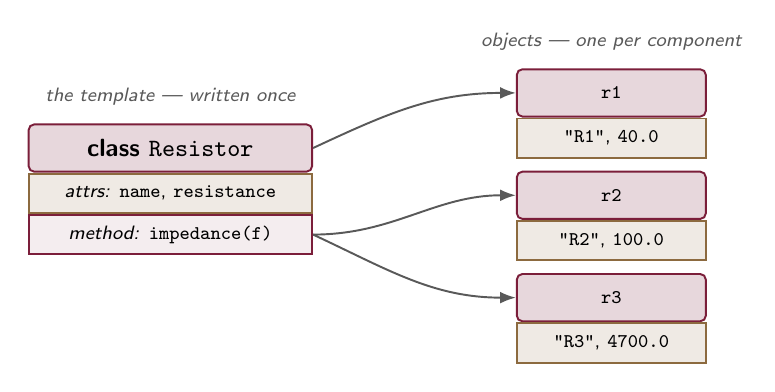
\begin{tikzpicture}
        \node[oopttl, minimum width=36mm] (cttl) at (0,0) {class \texttt{Resistor}};
        \node[oopdata, below=0mm of cttl, minimum width=36mm, anchor=north] (cd)
             {\textit{attrs:} \texttt{name}, \texttt{resistance}};
        \node[oopmeth, below=0mm of cd, minimum width=36mm, anchor=north] (cm)
             {\textit{method:} \texttt{impedance(f)}};
        \node[ooplbl, above=1.5mm of cttl] {the template --- written once};

        \node[oopttl, minimum width=24mm, font=\sffamily\bfseries\scriptsize]
             (o1) at (5.6,0.7) {\texttt{r1}};
        \node[oopdata, below=0mm of o1, minimum width=24mm, anchor=north] (o1d)
             {\texttt{"R1"}, \texttt{40.0}};

        \node[oopttl, minimum width=24mm, font=\sffamily\bfseries\scriptsize]
             (o2) at (5.6,-0.6) {\texttt{r2}};
        \node[oopdata, below=0mm of o2, minimum width=24mm, anchor=north] (o2d)
             {\texttt{"R2"}, \texttt{100.0}};

        \node[oopttl, minimum width=24mm, font=\sffamily\bfseries\scriptsize]
             (o3) at (5.6,-1.9) {\texttt{r3}};
        \node[oopdata, below=0mm of o3, minimum width=24mm, anchor=north] (o3d)
             {\texttt{"R3"}, \texttt{4700.0}};

        \node[ooplbl, above=1.5mm of o1] {objects --- one per component};
        \draw[ooparr] (cttl.east) to[out=25,in=180]  (o1.west);
        \draw[ooparr] (cm.east)   to[out=0,in=180]   (o2.west);
        \draw[ooparr] (cm.east)   to[out=-25,in=180] (o3.west);
    \end{tikzpicture}
    \end{center}
    {\scriptsize Each object gets its own copy of the data, but they share
    the one definition of \texttt{impedance()}.}
\end{frame}

%===============================================================================
\section{Adding Methods}
%===============================================================================

\begin{frame}[fragile]{A Method: a Function Defined Inside a Class}
    \leavevmode
    A class that only stores data is little better than a dictionary ---
    the point of an object is that it also carries the operations valid
    on that data:

\begin{lstlisting}
class Resistor:
    def __init__(self, name, resistance):
        self.name = name
        self.resistance = resistance

    def impedance(self, f):
        # A resistor's impedance is real, independent of frequency
        return complex(self.resistance, 0)

r1 = Resistor("R1", 40.0)
print(r1.impedance(1000))
\end{lstlisting}
    \texttt{(40+0j)}
\end{frame}

\begin{frame}{Reading the Method}
    \leavevmode
    \small
    The method takes \texttt{self} first, then its own arguments. Inside,
    it reaches the object's stored data through
    \texttt{self.resistance} --- no separate resistance parameter is
    needed, because the object already knows its own value.

    \vspace{3mm}
    \begin{block}{Calling it}
        \texttt{r1.impedance(1000)}: the object before the dot becomes
        \texttt{self}.
    \end{block}
\end{frame}

%===============================================================================
\section{Inheritance: Sharing Behaviour}
%===============================================================================

\begin{frame}{Resistors, Inductors, Capacitors: Mostly the Same}
    \leavevmode
    Each has a name and a value, each can report an impedance --- but
    each computes it differently (Chapter 8).

    \vspace{2mm}
    \begin{alertblock}{Rather than three unrelated classes with
        duplicated code \ldots}
        \ldots one class can be defined as a specialised version of
        another. This is \alert{inheritance}.
    \end{alertblock}
\end{frame}

\begin{frame}[fragile]{A Shared Base Class}
    \leavevmode
\begin{lstlisting}
class Component:
    """Shared behaviour for any two-terminal component."""
    def __init__(self, name, value):
        self.name = name
        self.value = value

    def impedance(self, f):
        raise NotImplementedError("Each type defines its own impedance")

    def describe(self, f):
        Z = self.impedance(f)
        return f"{self.name}: Z = {Z:.2f} ohm, |Z| = {abs(Z):.2f} ohm"
\end{lstlisting}
\end{frame}

\begin{frame}[fragile]{Three Subclasses, One Line Each}
    \leavevmode
\begin{lstlisting}
class Resistor(Component):
    def impedance(self, f):
        return complex(self.value, 0)          # Z = R

class Inductor(Component):
    def impedance(self, f):
        return 1j * 2 * np.pi * f * self.value  # Z = +j*w*L

class Capacitor(Component):
    def impedance(self, f):
        return -1j / (2 * np.pi * f * self.value)  # Z = -j/(w*C)
\end{lstlisting}

    \vspace{2mm}
    \begin{block}{What \texttt{class Resistor(Component)} declares}
        A \texttt{Resistor} \alert{is a} \texttt{Component}: it
        automatically gains \texttt{\_\_init\_\_} and \texttt{describe()}
        without repeating them. Replacing an inherited method is called
        \alert{overriding}.
    \end{block}
\end{frame}

\begin{frame}{What Is Shared, What Is Replaced}
    \leavevmode
    \begin{center}
    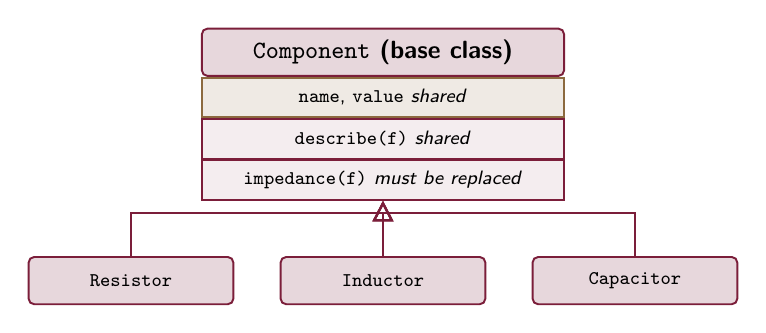
\begin{tikzpicture}
        \node[oopttl, minimum width=46mm] (bttl) at (0,0) {\texttt{Component} (base class)};
        \node[oopdata, below=0mm of bttl, minimum width=46mm, anchor=north] (bd)
             {\texttt{name}, \texttt{value} \hfill \textit{shared}};
        \node[oopmeth, below=0mm of bd, minimum width=46mm, anchor=north] (bm1)
             {\texttt{describe(f)} \hfill \textit{shared}};
        \node[oopmeth, below=0mm of bm1, minimum width=46mm, anchor=north] (bm2)
             {\texttt{impedance(f)} \hfill \textit{must be replaced}};

        \node[oopttl, minimum width=26mm, font=\sffamily\bfseries\scriptsize]
             (rt) at (-3.2,-2.9) {\texttt{Resistor}};
        \node[oopttl, minimum width=26mm, font=\sffamily\bfseries\scriptsize]
             (lt) at (0,-2.9) {\texttt{Inductor}};
        \node[oopttl, minimum width=26mm, font=\sffamily\bfseries\scriptsize]
             (ct) at (3.2,-2.9) {\texttt{Capacitor}};

        \draw[oopinh] (rt.north) -- ++(0,0.55) -| (bm2.south);
        \draw[oopinh] (lt.north) -- (bm2.south);
        \draw[oopinh] (ct.north) -- ++(0,0.55) -| (bm2.south);
    \end{tikzpicture}
    \end{center}
    {\scriptsize All three subclasses inherit \texttt{name}, \texttt{value},
    and \texttt{describe()} unchanged; each overrides \texttt{impedance()}
    with its own physics.}
\end{frame}

\begin{frame}[fragile]{The Payoff: Uniform Treatment}
    \leavevmode
\begin{lstlisting}
f = 60.0
circuit = [Resistor("R", 40.0), Inductor("L", 0.2), Capacitor("C", 50e-6)]

for c in circuit:
    print(c.describe(f))

Z_total = sum(c.impedance(f) for c in circuit)  # Series impedances add
print(f"Series total: Z = {Z_total:.2f} ohm")
\end{lstlisting}
\begin{lstlisting}[language={}]
R: Z = 40.00+0.00j ohm, |Z| = 40.00 ohm
L: Z = 0.00+75.40j ohm, |Z| = 75.40 ohm
C: Z = -0.00-53.05j ohm, |Z| = 53.05 ohm

Series total: Z = 40.00+22.35j ohm
\end{lstlisting}
\end{frame}

\begin{frame}{Check: Same Numbers, Different Organisation}
    \leavevmode
    \begin{block}{Check}
        These are the \alert{same numbers} computed in Chapter 8 for the
        same series RLC circuit: $Z = 40 + 22.35j\,\Omega$, magnitude
        $45.82\,\Omega$, phase $29.2^{\circ}$.
    \end{block}

    \vspace{3mm}
    The physics has not changed and the arithmetic has not changed. What
    changed is the \alert{organisation}: the loop over \texttt{circuit}
    does not know or care which kind of component it holds --- it simply
    asks each one for its impedance.

    \vspace{2mm}
    {\small Adding a fourth component type would require no change to
    that loop at all.}
\end{frame}

%===============================================================================
\section{EE Focus: Wrapping the Bench Recording}
%===============================================================================

\begin{frame}{Back to the Running Dataset}
    \leavevmode
    The second natural use of a class in this book: the recurring bench
    dataset. A \alert{Signal} object can hold a time axis and its
    samples, and carry the operations developed across earlier chapters
    (arrays, error handling, curve fitting).
\end{frame}

\begin{frame}[fragile]{The Signal Class}
    \leavevmode
\begin{lstlisting}
class Signal:
    """A time series of measurements, with operations valid on it."""
    def __init__(self, t, v, name="signal"):
        self.t = np.asarray(t, dtype=float)
        self.v = np.asarray(v, dtype=float)
        self.name = name

    def n_missing(self):
        return int(np.isnan(self.v).sum())

    def repair(self):
        gaps = np.isnan(self.v)
        if gaps.any():
            self.v[gaps] = np.interp(self.t[gaps], self.t[~gaps], self.v[~gaps])
        return self

    def time_constant(self):
        return -1 / np.polyfit(self.t, np.log(self.v), 1)[0]
\end{lstlisting}
\end{frame}

\begin{frame}[fragile]{Using It}
    \leavevmode
\begin{lstlisting}
t = np.arange(0, 2.001, 0.02)
v = 12.0 * np.exp(-t / 0.47)
v[40:43] = np.nan          # the three samples the logger lost near t=0.8 s

rc = Signal(t, v, name="bench_rc voltage")
print(rc.summary())

rc.repair()
print(rc.summary())
print(f"Measured tau: {rc.time_constant():.4f} s")
\end{lstlisting}
\begin{lstlisting}[language={}]
bench_rc voltage: 101 samples, 3 missing, v from 12.00 to 0.17 V
bench_rc voltage: 101 samples, 0 missing, v from 12.00 to 0.17 V
Measured tau: 0.4700 s
\end{lstlisting}
\end{frame}

\begin{frame}{When Does This Earn Its Keep?}
    \leavevmode
    Everything this class does was already possible with plain functions
    --- for a single recording, the plain version is perfectly
    reasonable.

    \vspace{3mm}
    \begin{alertblock}{The organisation earns its keep when \ldots}
        \ldots there are \alert{several} recordings: voltage, current,
        and temperature from the same logger, or the same experiment
        repeated at three temperatures. Each becomes its own
        \texttt{Signal}, and no call can accidentally pair one
        recording's samples with another's time axis.
    \end{alertblock}
\end{frame}

\begin{frame}{A Caution About Mutation}
    \leavevmode
    \texttt{repair()} modifies \texttt{self.v} \alert{in place}, so the
    original samples are overwritten.

    \vspace{3mm}
    \begin{block}{A genuine design decision, not an accident of syntax}
        Convenient --- but the raw measurement is gone. Chapter 11
        argued that repairs should be \alert{documented}, not silent.
    \end{block}

    \vspace{2mm}
    {\small Where the unrepaired data must be preserved, the method
    should instead return a \emph{new} \texttt{Signal} and leave the
    original untouched.}
\end{frame}

%===============================================================================
\section{When to Use a Class --- and When Not To}
%===============================================================================

\begin{frame}{A Tool With a Specific Purpose}
    \leavevmode
    OOP is not a better way to write everything. For the engineering
    calculations in this book, plain functions and NumPy arrays are
    usually the clearer choice.

    \vspace{3mm}
    \begin{block}{A class is worth defining when \ldots}
        \begin{itemize}\itemsep2pt
            \small
            \item Several pieces of data always belong together.
            \item A set of operations only makes sense on that
                  particular data.
            \item You need several independent copies of the same kind
                  of thing.
            \item Related kinds of thing share most of their behaviour
                  and differ in a little of it.
        \end{itemize}
    \end{block}
\end{frame}

\begin{frame}{A Plain Function Is Usually Better}
    \leavevmode
    When the operation is a self-contained calculation that takes inputs
    and returns an output --- which describes \alert{most} of what an
    engineer computes.

    \vspace{2mm}
    {\small Converting units, fitting a curve, integrating a signal: none
    of these need a class.}

    \vspace{4mm}
    \begin{alertblock}{Why learn objects anyway?}
        The libraries central to engineering computation are built from
        them. Every \texttt{arr.mean()}, \texttt{df.groupby()}, or
        \texttt{ax.set\_xlabel()} is a method call on an object. Knowing
        this turns documentation from a list of incantations into
        something you can reason about.
    \end{alertblock}
\end{frame}

%===============================================================================
\section{Summary}
%===============================================================================

\begin{frame}{Summary}
    \leavevmode
    \small
    \begin{itemize}\itemsep3pt
        \item A \alert{class} is a template; an \alert{object} is one
              instance built from it. NumPy arrays and pandas DataFrames
              are objects --- hence \texttt{a.mean()}, not
              \texttt{mean(a)}.
        \item \texttt{\_\_init\_\_} runs automatically on creation and
              sets up starting data. Never called directly.
        \item \texttt{self} refers to the particular object a method is
              working on. \texttt{self.something} values are
              \alert{attributes}.
        \item A \alert{method} is a function defined inside a class,
              reaching the object's data through \texttt{self}.
        \item \alert{Inheritance} lets a class reuse another's behaviour
              and replace only what differs (\alert{overriding}).
        \item Objects organise code; they do not change the mathematics.
        \item Use a class when data and operations genuinely belong
              together. Use a plain function otherwise --- which covers
              most engineering computation.
    \end{itemize}
\end{frame}

\begin{frame}{Where This Is Going}
    \leavevmode
    \small
    This chapter is enrichment --- the core path through the book does
    not require writing your own classes.

    \vspace{3mm}
    \begin{itemize}
        \item You will keep \alert{using} objects constantly: every
              NumPy array, every pandas DataFrame, every Matplotlib axis.
        \item Chapter 16's mini-projects return to plain functions and
              arrays, the everyday tools of this course.
        \item If a future project grows large enough that several
              recordings must travel with their own rules, you now know
              the tool that organises it.
    \end{itemize}

    \vspace{4mm}
    \begin{center}
        \large\color{primary}\textbf{Next: Engineering Mini-Projects}
    \end{center}
\end{frame}

\end{document}
